\documentclass{article}
\usepackage[T1]{fontenc}
\usepackage{lmodern}
\usepackage{graphicx}
\usepackage{amsmath,amssymb}
\usepackage[a4paper,margin=2cm]{geometry}
\usepackage[absolute,overlay]{textpos}
\setlength{\TPHorizModule}{1mm}
\setlength{\TPVertModule}{1mm}
\usepackage[indonesian]{babel}
\usepackage{hyperref}
\setlength{\emergencystretch}{2em}
% unit: Halaman 25

\begin{document}

% === Halaman 25 (llm) ===

Contoh: kriptogram XMZVH

\vspace{5mm}

Plainteks yang potensial adalah CREAM dengan $k = 21$.
Kunci ini digunakan untuk mendekripsikan potongan cipherteks lainnya.

% deskripsi: Tabel contoh exhaustive key search terhadap cipherteks XMZVH yang menunjukkan berbagai kunci (k) ciphering dan hasil dekripsinya.
% bbox normalisasi: [0.1610, 0.2500, 0.8140, 0.6810]
\begin{textblock*}{137.13mm}(33.81mm,74.25mm)
\noindent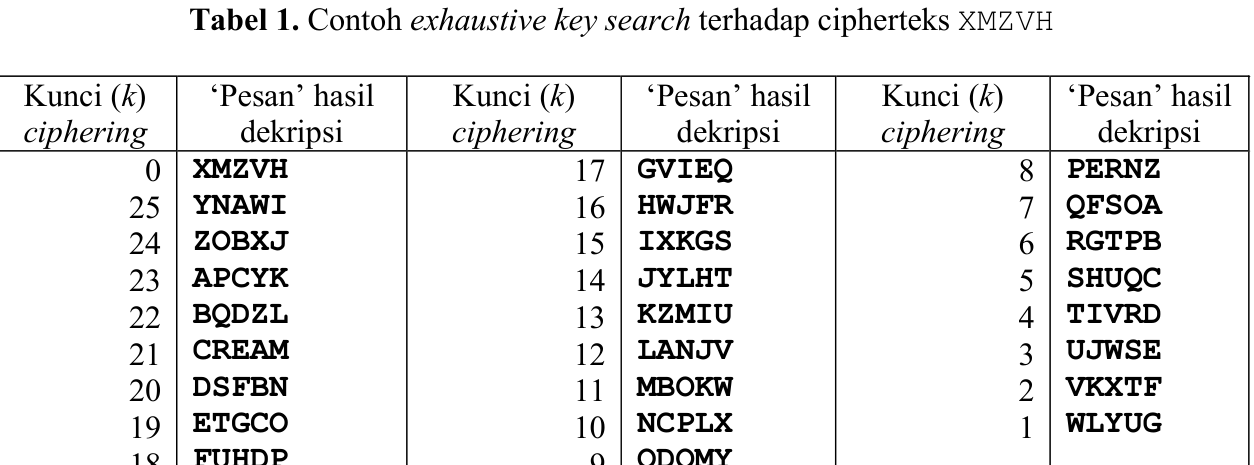
\includegraphics[width=137.13mm,height=128.01mm]{../../images/llm/page_025_img_01.png}%
\end{textblock*}

\end{document}
